\documentclass{beamer}
\setbeamertemplate{footline}[frame number]
%\usepackage{beamerthemeBerkeley}
\usetheme{Montpellier}
%\usetheme{Warsaw}
%\usetheme{Boadilla}
\usepackage[english]{babel}
\usepackage{graphicx}
%\usepackage{ams}
%\usepackage{blue}
\usepackage{amsmath} 
\usepackage{xcolor}
\usepackage{color}

\definecolor{red}{rgb}{1,0,0}
\def\Red{\color{red}}
\def\blue{\color{blue}}
\definecolor{blue2}{rgb}{0.1,0,0.55}
\definecolor{DarkGreen}{rgb}{0,0.5,0}
\def\DarkGreen{\color{DarkGreen}}


\newcommand{\myp}{\ensuremath{\mathbb{P}}}
\newcommand{\mye}{\ensuremath{\mathbb{E}}}
\newcommand{\myvar}{\mathbf{Var}}
\newcommand{\mycov}{\mathbf{Cov}}
\newcommand{\myind}{\ensuremath{\mathbbm{1}}}

\newcommand{\mI}{\ensuremath{\pmb{\mathsf{I}}}}
\newcommand{\mL}{\ensuremath{\pmb{\mathsf{L}}}}
\newcommand{\mQ}{\ensuremath{\pmb{\mathsf{Q}}}}
\newcommand{\mV}{\ensuremath{\pmb{\mathsf{V}}}}
\newcommand{\mW}{\ensuremath{\pmb{\mathsf{W}}}}
\newcommand{\mX}{\ensuremath{\pmb{\mathsf{X}}}}
\newcommand{\mZ}{\ensuremath{\pmb{\mathsf{Z}}}}

\newcommand{\ba}{\mathbf{a}}
\newcommand{\bd}{\mathbf{d}}
\newcommand{\bg}{\mathbf{g}}
\newcommand{\bV}{\mathbf{V}}
\newcommand{\bX}{\mathbf{X}}
\newcommand{\bY}{\mathbf{Y}}
\newcommand{\bZ}{\mathbf{Z}}

\newcommand{\bzero}{\mathbf{0}}

\newcommand{\balpha}{\mbox{\boldmath$\alpha$}}
\newcommand{\bbeta}{\mbox{\boldmath$\beta$}}
\newcommand{\bepsilon}{\mbox{\boldmath$\epsilon$}}
\newcommand{\bgamma}{\mbox{\boldmath$\gamma$}}
\newcommand{\bDelta}{\mbox{\boldmath$\Delta$}}
\newcommand{\bPhi}{\mbox{\boldmath$\Phi$}}
\newcommand{\bPsi}{\mbox{\boldmath$\Psi$}}
\newcommand{\bSigma}{\mbox{\boldmath$\Sigma$}}
\newcommand{\bmu}{\mbox{\boldmath$\mu$}}



\title{Lecture 7: Rare Variant Analysis: Collapsing Tests, Kernel (Variance Component) Tests and Omnibus Tests}

\author{Instructors: Joelle Mbatchou and Loic Yengo} 


\date{}


\begin{document}
	
	
	\begin{frame}
		\titlepage
		\vspace{-2cm}
		\begin{center}
			
			{ \Large Summer Institute in Statistical Genetics 2022\\}
			
			
		\end{center}
	\end{frame}


\begin{frame}
\frametitle{\bf Lecture Overview}

\begin{enumerate}
\item Limitations of GWAS 
\item Rationale for Rare Variant Analysis
\item Challenges
\item Collapsing/Burden Tests 
\item Variance Component Tests 
\item Omnibus Tests
\end{enumerate}
\end{frame}

\section{Limitations of GWAS}

\frame{
\frametitle{GWAS: Missing Heritability}
\begin{itemize}
\item GWAS primarily focus on { common} variants (MAF $\geq$ 5\%) whose effects are
		 small.
	\item {\bf Missing heritability:} Significant GWAS SNPs explain  a small proportion of disease heritability.
	\item Possible reasons: 
	\begin{itemize}
		\item GxG and GxE interactions?
		\item Many common causal variants: Each with a small effect?
		\item Epigenetics?
		\item {\bf Rare variants?}
	\end{itemize}
\end{itemize}
}

\section{Rationale for Rare Variant Analysis}

\frame{
	\frametitle{Why rare variants?} 
\begin{minipage}{.45\textwidth}
\begin{itemize}
\item Most of human variants are rare.
\item Functional variants tend to be rare.
	\end{itemize}
\end{minipage}% This must go next to `\end{minipage}`
\begin{minipage}{.55\textwidth}
	\begin{figure}
		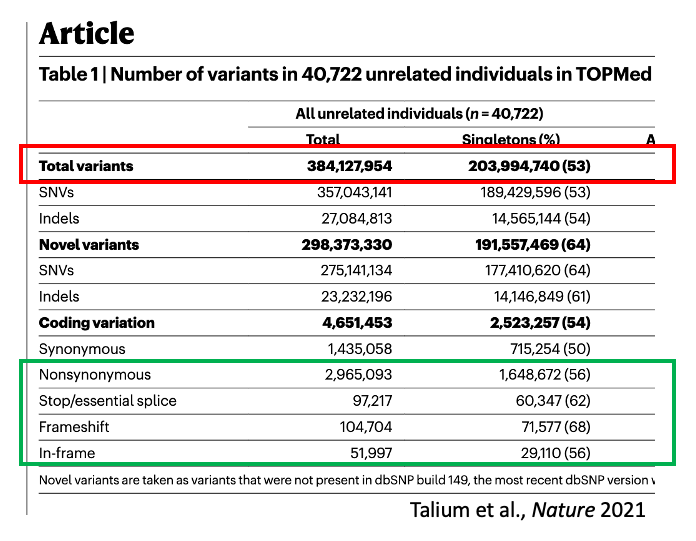
\includegraphics[scale=.35]{Figures/topmed}
	\end{figure}
\end{minipage}
}
 

\section{Challenges}

\frame{\frametitle{Challenges in Association Studies for Rare Variants}

\begin{itemize}

      	\item Compared to common variant studies, {\bf individual SNP analysis in rare variant studies is seriously underpowered.}
$\rightarrow$ How many subjects are needed to achieve $80\%$ of power ($\alpha = 10^{-6}$) by single variant test?

\begin{center}
	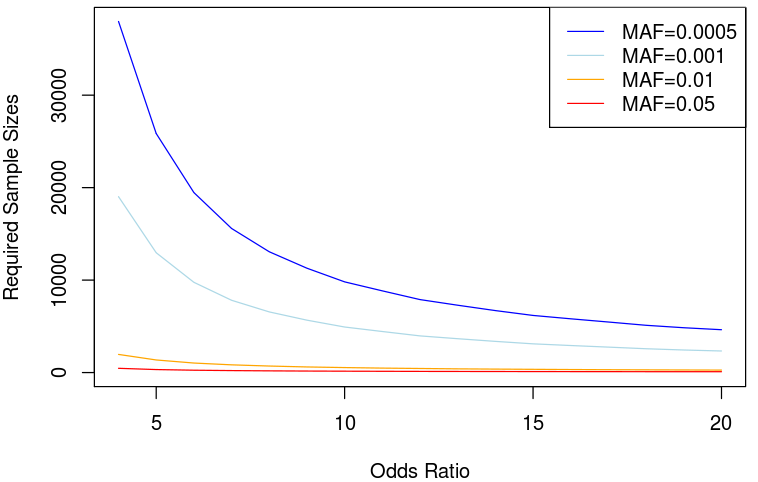
\includegraphics[scale=.35]{./Figures/PIC_Power_Single}
\end{center}
	\item A lot more rare variants than common variants $\rightarrow$ larger multiple testing burden
\end{itemize}
}




\frame{\frametitle{Challenges in Association Studies for Rare Variants}

\begin{itemize}
      \item Individual rare variant tests are underpowered
      \bigskip
     
      \item Need {\bf cost-effective study designs} to genotype a large number of individuals
      
      \bigskip
      \item Need {\bf powerful statistical methods and strategies} to test for associations
      
      \begin{itemize}
      \item Region based analysis: genes, moving windows, networks/pathways
      
      \item Integrate with bioinformatics: Incorporate functional information
      
      \end{itemize}

\end{itemize}
}

\section{Region Based Testing Strategy}

\frame{\frametitle{Region Based Analysis of Rare Variants} 
\begin{itemize}

  \item Gene (or Region) based tests 
  \item  Strategy:

   \begin{itemize}
      \item Identify all observed variants within a sequenced (sub)-region.
      \item Regions: gene, regulatory region, ...
      \item Test the joint effect  of rare/common variants.
    \end{itemize}
\end{itemize}

}


\frame{\frametitle{Regression Models} 
\begin{itemize}
	\item $p$ variants in a certain region.
	\item { SNPs in a region} ${\bf G_i}= (g_{i1}, g_{i2}, \ldots, g_{ip})'$, $(g_{ij} = 0,1, 2)$
	\item { Covariates} $\bX_i$ : age, gender, PC scores (for population stratification).
	\item Continuous/binary traits: 
	$$ g(\mu_i)=\alpha_0  + \bX_i' \balpha + \bf G_i' \bbeta    $$
	\item Joint test of no genetic  effect in region:
	$$H_0: \bbeta =(\beta_1,\ldots, \beta_p)= 0$$
\end{itemize}

}

\frame{
  \frametitle{Major Classes of Tests}
  \begin{itemize}
  	\item Burden/Collapsing tests
  	\item Supervised/Adaptive Burden/Collapsing tests
  	\item Variance component (similarity) based tests
  	\item Omnibus tests
  \end{itemize}
 }


\section{Collapsing/Burden Tests}

\frame{\frametitle{Collapsing/Burden Tests - Principle} 

\begin{itemize}\setlength{\itemsep}{1.1ex}
  \item  If $p$ is large, multivariate test $\bbeta = 0$ is not powerful (df=$p$). 
  \item  {Collapsing}: Suppose $\beta_1 = \cdots= \beta_p = \beta$
  \begin{align*}
  	g(\mu_i)&=\alpha_0  + \bX_i' \balpha + \bf G_i' \bbeta \\
  	&=\alpha_0  + \bX_i^T \balpha + C_i \beta 
  \end{align*}
 
 \item $C_i = g_{i1} + \cdots + g_{ip}$ : {\bf genetic burden/score}
 \item Test $H_0: \beta = 0 $ (df=1)
 	\item  {\bf Key assumption}: all rare variants  in region are causal variants with the same effect sizes and association directions. 
\end{itemize}
}


\frame{\frametitle{Burden Tests} 

\begin{itemize}\setlength{\itemsep}{1.1ex}
  \item Collapse rare variants
\end{itemize}

\begin{center}
\begin{figure}
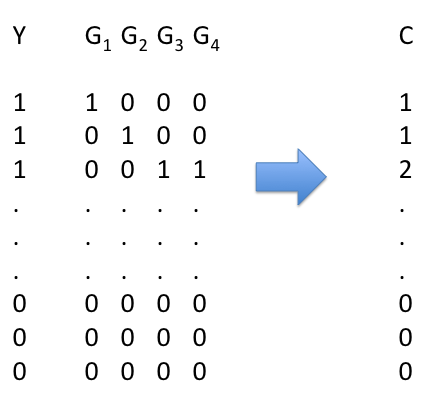
\includegraphics[scale=.35]{./Figures/Slide2}
\end{figure}
\end{center} 

}



\frame{\frametitle{Burden Tests} 

\begin{itemize}\setlength{\itemsep}{1.1ex}
  \item  Many different types of tests exist based on different  aggregation rules to get $C_i$
  \begin{itemize}
  	\item Reflects assumptions on genetic architecture
  \end{itemize}
  \item  {\bf Existence of any rare variants can cause loss of function of a region} (e.g. CAST)
$$ C_i = \left\{
\begin{array}{ll}
   1 & \textrm{if} \quad \sum\limits_{j=1}^{p} g_{ij} > 0 \\
   0 & \textrm{if} \quad \sum\limits_{j=1}^{p} g_{ij} = 0 \\
\end{array} \right. $$  
 \item  {\bf Dominant genetic model} (e.g.. MZ-test)
$$ C_i =  \sum\limits_{j=1}^{p} I(g_{ij} > 0)$$

\end{itemize}
}



\frame{\frametitle{Weighted Burden} 


\begin{itemize}\setlength{\itemsep}{1.2ex}
  \item Assume that {\bf rarer variants have larger effects}
  \item Suppose $\beta_j = w_j \beta$, where $w_j =  w (MAF_j) $. 
  \begin{itemize}
  \item Ex: $w(MAF_j) = 1/\sqrt{MAF_j(1-MAF_j)}$ (Madsen and Browning). 
  \end{itemize}
  \item Weighted count of rare variants
  $$C_i = w_1 g_{i1} + \cdots + w_p g_{ip}$$
\end{itemize}
}



\frame{\frametitle{Power of Burden Tests} 
\begin{itemize}\setlength{\itemsep}{1.2ex}
	\item Power of burden tests depends on 
		\begin{itemize}
			\item Number of  associated variants
			\item Number of  non-associated variants
			\item Direction of the effects.
		\end{itemize}
			
					
			\item \textbf{Powerful if most variants are causal and have effects in the same direction.}
\end{itemize}

}




\section{Rare variants test: Variance component test}

\frame{\frametitle{Variance component  test} 
	
	\begin{itemize}\setlength{\itemsep}{1.2ex}
		\item Burden tests are not powerful, if  
		\begin{itemize}
			\item there exist variants with different association directions 
			\item many non-causal variants
		\end{itemize}
		
		\item Variance component tests have been proposed to address this limitation.
		
	\end{itemize}
}





\frame{\frametitle{Sequence Kernal Association Test (SKAT)} 
%		{\large Wu et al., (2010, 2011).  {\it AJHG}}
	
	\begin{itemize}\setlength{\itemsep}{1.2ex}
		% \item {\bf Variance component test} under the regression model
		\item Recall the original  regression models:
		\begin{align}
			& g(\mu_i)= \alpha_0  + \bX_i^T \balpha + {\bf G}_i^T \bbeta \notag 
		\end{align}
		%\item LR test of $\bbeta = 0$ has little power with a large $p$.
			\item Assume $\beta_j \sim dist. (0, w_j^2 \tau)$.
			\item $H_0: \beta_1 = \cdots = \beta_p = 0 \iff  H_0: \tau = 0 $.
			\item 1df test!
	\end{itemize}
}


\frame{\frametitle{Sequence Kernel Association Test (SKAT)} 
	
	
	\begin{itemize}\setlength{\itemsep}{1.1ex}
		\item Score test statistic for $\tau = 0$:
		$$ Q_{SKAT} = ( {\bf y} - {\boldsymbol {\hat{\mu}}} _0  )' {\bf K}( {\bf y} - {\boldsymbol {\hat{\mu}}} _0  ), $$
		\item ${{\bf K} = {\bf G } {\bf W }{\bf W } {\bf G }'}$ : weighted linear kernel (where ${\bf W }= diag[w_1,\ldots, w_p]$).
		\item It is a $N\times N$ similarity matrix 
		
	\end{itemize}
}


\frame{\frametitle{SKAT}
	
	\begin{itemize}
		\item $Q_{SKAT}$ is a {\bf weighted sum of single variant score statistics}
		\begin{align}
			Q_{SKAT} & = ( {\bf y} - {\boldsymbol {\hat{\mu}}} _0   )' {\bf G } {\bf W }{\bf W } {\bf G }' ( {\bf y} - {\boldsymbol {\hat{\mu}}} _0  ) \notag \\
			& = \sum_{j=1}^p w_j^2 [ \bg_j'  ({\bf y} - {\boldsymbol {\hat{\mu}}} _0  )] = \sum_{j=1}^p w_j^2 S_j^2 \notag
		\end{align}
%		where $U_j = \sum_{i=1}^n g_{ij} (y_i - \muhat_{0i}) $.
		\item $S_j$ is a score test statistic in the SNP $j$ only model:
		{  $$g(\mu_i)= \alpha_0  + \bX_i^T \balpha + g_{ij} \beta_j   $$}
			\item Under $H_0$, $Q_{SKAT}$ (asymptotically) follows a {\bf mixture of $\chi^2$ distribution} $ \sum_{j=1}^p \lambda_j \chi^2_{1,j}$
	\end{itemize}
}


\frame{\frametitle{Burden vs SKAT}
	
	\begin{itemize}
		\item Power simulations: 5\% of the variants in region are causal \& vary the directions of effects
		\item SKAT remains powerful even if variants have different effect directions
		\vspace{-1em}
		\begin{figure}
			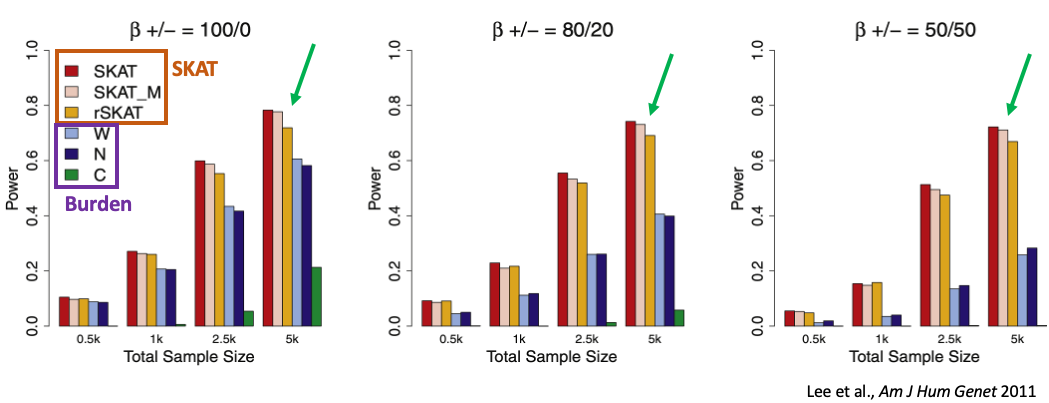
\includegraphics[scale=.35]{./Figures/burden_skat}
		\end{figure}
		
	\end{itemize}
}



\section{Omnibus Tests}



\frame{
	\frametitle{SKAT vs. Collapsing}
	\begin{itemize}
		\item Collapsing tests are more powerful when a large \% of variants are causal and effects are in the same direction.
		\item SKAT is more powerful when a small \% of variants are causal, or the effects have mixed directions.
		\item Both scenarios can happen when scanning the genome.
		\item Best test to use depends on the underlying biology.
		\begin{center}
			$\rightarrow$ Difficult to choose which test to use in practice.
		\end{center}
	\vspace{0.4cm}
\pause
{\bf We want to develop a unified test that works well in both situations $\rightarrow$ Omnibus tests}
	\end{itemize}
}


\frame{\frametitle{Combine Test Statistics: Unified Test Statistics} 
	
	\vspace{-0.15in}
	\begin{center}
		{\large Lee (2012).  {\it Biostatistics}}
	\end{center}
	\begin{itemize}
		\item Combined Test of Burden tests and SKAT
		{\blue 	$$ Q_\rho = (1 -\rho) Q_{SKAT} + \rho Q_{Burden}, \quad  0 \leq \rho \leq 1. $$}
	\end{itemize}
	
	\begin{itemize}
		%\item $\rho=0$ $\Rightarrow$ SKAT.
		\item $Q_{\rho}$ includes SKAT and burden tests.
		\begin{itemize}
			\item $\rho=0$: SKAT
			\item $\rho=1$: Burden
		\end{itemize}
	\end{itemize}
	
	
}
\frame{\frametitle{SKAT-O} 
	\begin{itemize}
		\item { Model}:
		$$	g(\mu_i)= \alpha_0  + \bX_i^T \balpha + {\bf G}_i^T \bbeta \notag $$
		where  $\beta_j / w_j$ follows any arbitrary distribution  with mean 0 and variance $\tau$
		and {\blue the correlation among $\beta_j$'s is $\rho$}.
		\item Special cases:
		\begin{itemize}
			\item SKAT: $\rho=0$
			\item Burden: $\rho=1$
		\end{itemize}
		% \item $\rho$ is  a correlation among $\beta$
		\item Set a grid of values for $\rho$  in $[0,1]$ and pick $\rho$ which maximizes power
		\item SKAT-O p-value is obtained through numerical integration
	\end{itemize}
}

\frame{\frametitle{SKAT-O vs Burden/SKAT}
	
	\begin{itemize}
		\item SKAT-O remains powerful across all scenarios
		\begin{figure}
			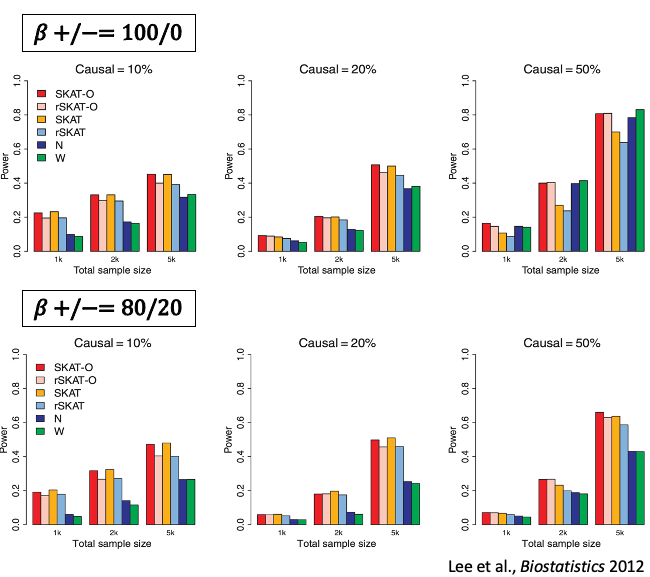
\includegraphics[scale=.35]{./Figures/burden_skat_skato}
		\end{figure}
		
	\end{itemize}
}


\frame{\frametitle{Aggregated Cauchy Association Test: ACAT} 
	\begin{itemize}
		\item Based on the Cauchy combination method to combine a set of p-values $\{p_j\}$:
		$$ T_{ACAT} = \sum_j w_j \tan\{\pi(0.5-p_j)\} $$
		\item Computing p-value is extremely fast 
		$$ \text{p-value}\approx 0.5 - \frac{\arctan\{T_{ACAT}/w\} }{\pi}, \quad w=\sum_j w_j$$
		\item Insensitive to correlation in the p-values (can be unknown)
	\end{itemize}
}


\frame{\frametitle{Aggregated Cauchy Association Tests} 
	\begin{itemize}
		\item ACAT-V
				\begin{itemize}
			\item Apply ACAT to single variant p-values from rare variants
	\item More powerful when fewer variants are associated (i.e. sparse alternative)
	\item SKAT \& Burden can loose substantial power under this scenario
		\end{itemize}
	\item ACAT-O
				\begin{itemize}
\item Apply ACAT to combine the p-values of SKAT, Burden and ACAT-V
		\item Omnibus test which should work well whether 
		\begin{itemize}
			\item Effects are in same direction \& many variants are associated
			\item Effects are in different directions
			\item Very few variants are causal
		\end{itemize}
\end{itemize}
		\end{itemize}
}


\frame{\frametitle{ACAT/SKAT/Burden }
	
	\begin{itemize}
		\item ACAT-O remains powerful across all scenarios
		\begin{figure}
			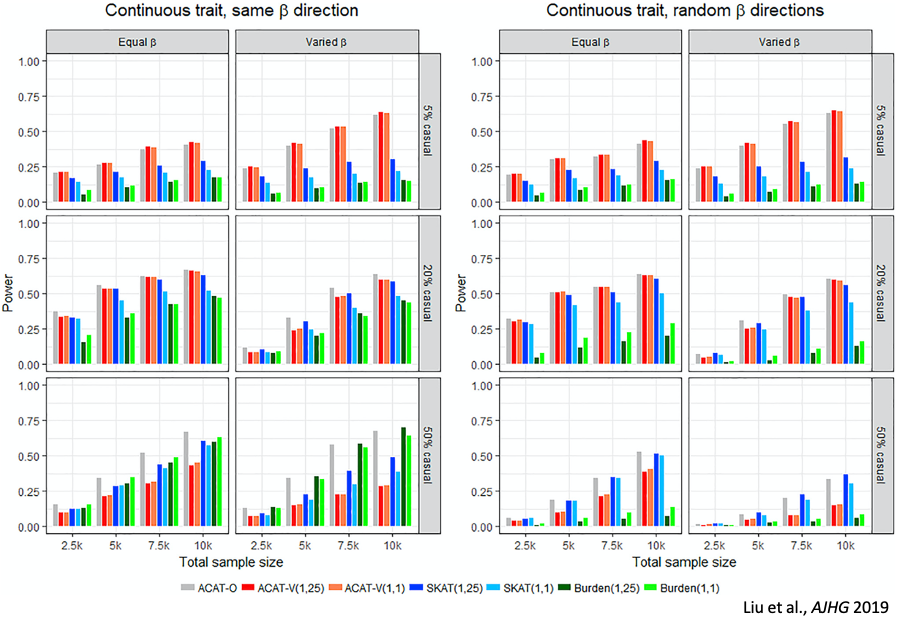
\includegraphics[scale=.33]{./Figures/acat_skat_burden}
		\end{figure}
		
	\end{itemize}
}



%\subsection{Summary}
\frame{\frametitle{Takeaways} 
	
	\begin{itemize}
		\item Region based tests can increase the power of rare variants analysis compared to single variant tests.
		\item Relative performance of rare variant tests depends on underlying disease models 
		\item  Combined tests (omnibus tests), e.g, SKAT-O/ACAT-O, are more robust and powerful across different scenarios 
	\end{itemize}
	
	
}


\section{References}
\frame{\frametitle{References} 
	
	\begin{itemize}
		\item Taliun, D. et al. Sequencing of 53,831 diverse genomes from the NHLBI TOPMed Program. \textit{Nature} \textbf{590}, 290-299 (2021).
		\item Madsen, B.E. \& Browning, S.R. A Groupwise Association Test for Rare Mutations Using a Weighted Sum Statistic. \textit{PLoS Genetics} \textbf{5}, e1000384 (2009).
	\item 	Wu, M.C. et al. Rare-variant association testing for sequencing data with the sequence kernel association test. \textit{Am J Hum Genet} \textbf{89}, 82-93 (2011).
		\item Lee, S., Wu, M.C. \& Lin, X. Optimal tests for rare variant effects in sequencing association studies. \textit{Biostatistics} \textbf{13}, 762-75 (2012).
	\item 	Liu, Y. et al. ACAT: A Fast and Powerful p Value Combination Method for Rare-Variant Analysis in Sequencing Studies. \textit{Am J Hum Genet} \textbf{104}, 410-421 (2019).
		
	\end{itemize}
	
	
}



\end{document}
